% Created 2022-12-23 Fr 22:43
% Intended LaTeX compiler: pdflatex
\documentclass[20pt]{extarticle}
\usepackage[utf8]{inputenc}
\usepackage[T1]{fontenc}
\usepackage{graphicx}
\usepackage{longtable}
\usepackage{wrapfig}
\usepackage{rotating}
\usepackage[normalem]{ulem}
\usepackage{amsmath}
\usepackage{amssymb}
\usepackage{capt-of}
\usepackage{hyperref}
\usepackage{color}
\usepackage{listings}
\usepackage[english, germanb]{babel}
\usepackage[left=2.0cm,right=2.0cm,top=2.5cm,bottom=2.0cm]{geometry}
\makeatother
\usepackage{venturis2}
\usepackage{titlesec}
\usepackage{fancyhdr}
\newcommand{\sectionbreak}{\newpage\newpage\clearpage}
\graphicspath{{figures/}}
\usepackage{lettrine}
\usepackage{GoudyIn}
\renewcommand{\LettrineFontHook}{\GoudyInfamily{}}
\newcommand{\cb}[2]{\lettrine[lines=3]{#1}{#2}}
\renewcommand\thesection{}
\renewcommand\thesubsection{}
\usepackage{afterpage}
\newcommand\myemptypage{
\null
\thispagestyle{empty}
\addtocounter{page}{-1}
\newpage
}
\date{}
\title{Simons \\ Weihnachtsgeschichte \\ 2022}
\hypersetup{
 pdfauthor={},
 pdftitle={Simons \\ Weihnachtsgeschichte \\ 2022},
 pdfkeywords={},
 pdfsubject={},
 pdfcreator={Emacs 28.1 (Org mode 9.5.2)}, 
 pdflang={Germanb}}
\begin{document}

\begin{titlepage}
\centering
{\huge Simons \\ Weihnachtsgeschichte \\ 2022 \par }
\vspace{2cm}
{\large  \par}
\vspace{3cm}
\begin{figure}[h]\hspace*{-0.73cm}\begin{center}
\includegraphics[width=0.5\columnwidth]{santa}\end{center}\end{figure}\end{titlepage}
\setlength\parindent{0pt}


\section{Vorwort}
\label{sec:org5f96c74}
\cb{A}{lle} Jahre wieder fällt mir nicht ein, was ich den Leuten
schenken soll. Daher öffne ich mir eine Flasche Wein oder 2 und
stümper 20 Seiten Unsinn zusammen, die ich dann als Beschenkung
unter das Volk bringe.  \newline

Hi, falls du lieber Leser zum ersten mal in den zweifelhaften Genuss
kommst mit meiner Weihnachtsgeschichte bedacht zu werden oder
selbige trotz vorheriger Belästigung nun zum ersten mal liest,
möchte ich dir kurz die Spielregeln erklären. Simons saucoole
Sweihnachtsgeschichte ist ein Machwerk, das nur die Besten der
Besten der Besten zu sehen, hören und ja auch zu lesen
bekommen. Ich, meines zeichens the author, verpflichte mich wie
jedes Jahr dazu die Wahrheit und nur die Wahrheit zu Papier zu
bringen. Und dann kurz vor Weihnacht tippe ich irgendwelchen
erfundenen Quatsch am Computer und nenne es
\emph{Weihnachtsgeschichte}. Selbige, werter Leser haltet Ihr nun in
deinen Händen, Madame. So jetzt haben sich hoffentlich alle
angesprochen und respektiert gefühlt.
\newline

In guter Weihnachtsgeschichtentradition teilt sich die Geschichte in
mehrere Kapitel, jedes erfundener, ich meine spannender als das
zuvor kommende. Nun abandone all your hopes, schnall you an und
taucht ein into the void bzw. the Weihnachtsgeschichte.

\begin{center}
Fröhliche Weihnachten \\
und \\
einen guten Rutsch ins Jahr 2023.
\end{center}

\begin{center}
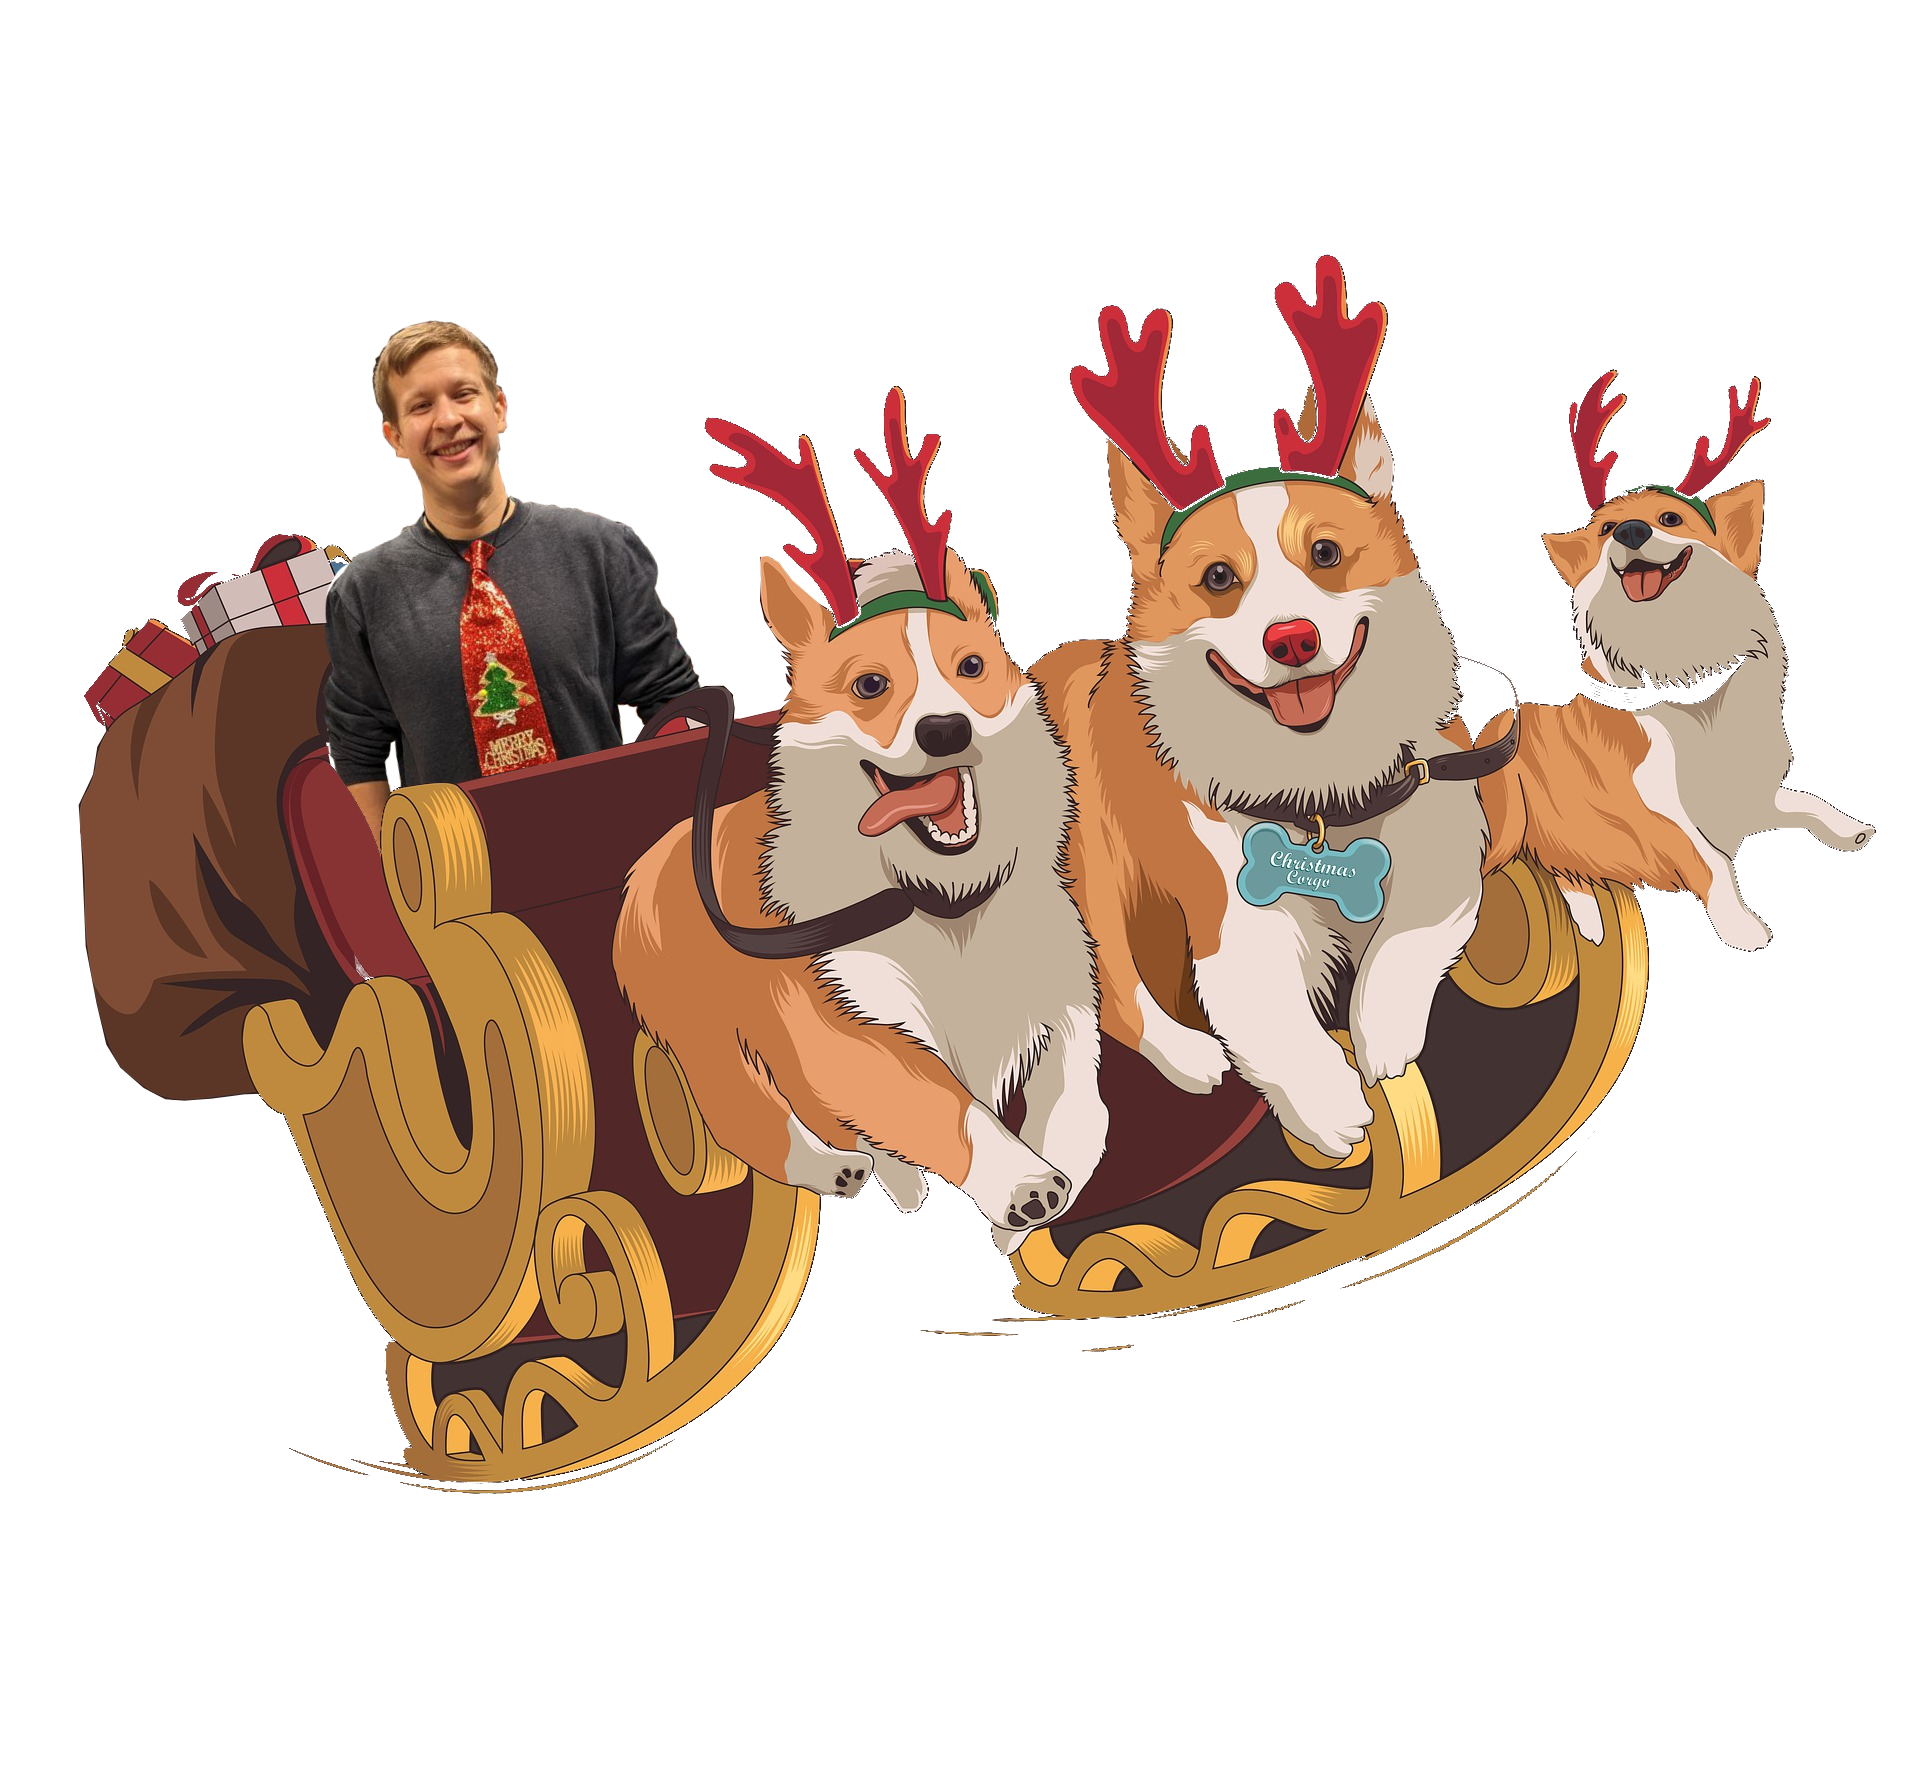
\includegraphics[height=18cm]{figures/simon2.png}
\end{center}
\section{Dem Stress entfliehen}
\label{sec:orgb7a853e}
\cb{D}{ie} S-Bahn wird langsamer. Auf der Anzeigetafel verkündet das
Infotainmentsystem meine Haltestelle. Endlich. Ungeduldig drücke ich
schon provisorisch den Türknopf, aber natürlich hilft das
nicht. Erst kommt der Zug frustrierend langsam zum stehen, dann
vergehen noch 1,2 Schweigesekunden, bis der LED ring um den Türknopf
grün leuchtend meinen Befehl annimmt. Ich springe regelrecht ins
Freie. Knirschend im Slalom schlängele ich mich durch die viel zu
langsamen Menschen auf dem Bahnsteig. Die Treppen runter. Halt!
Fahrräder von links und rechts, ich schnaube genervt. Aber dann,
300meter, 200, 50. Schlüssel ins fieselige Hoftürschloss,
Sicherheitsschlüssel an der Haustür, mit Gewalt die klemmende
Wohnungstür aufdrücken. Uff. \newline

Meine eigenen vier Wände begrüßen mich mit dem Düften von
unabgespülten Töpfen und den darin befindlichen Essensresten. Die
Heizung rattert, die habe ich wohl vergessen heute Früh
auszuschalten. Seufzend ergebe ich armes Kind mich meinem
schrecklichen Schicksal und mache Klarschiff. Fenster auf, Geschirr
spülen und trocken. Dann Wäsche gewaschen, Staubgesaugt ach ja klar
das Bad will geputz werden, klar doch. Trocke Wäsche abnehmen,
zusammenlegen veräumen. Gewaschene Wäsche
aufhängen. \newline

Ich bin endlich fertig und frisch gekochte Kaffee duftet
verführerisch. Finally, kann ich den Computer starten die Uni
Blätter warten. Oder ja, wie wär es mit Homeoffice das E-Mail
Programm begrüßt mich freudig piepend 30ungelesenen Nachrichten. Ich
will es gar nicht wissen, aber Discord, Whatsapp und Telegramm sind
auch begeistert, dass ich da bin. In einer besseren Welt hätten wir
alle einen Angestellten, der nichts anderes macht als den ganzen Tag
unsere Nachrichten zu lesen und zu beantworten. Am besten in so
einem richtig schön kurz angebundenem passiv aggrresiven Ton: "Nein"
\dots{} "Ja" \dots{} "Have you tried to turn it on and off again?"
\newline

Mir ist das jetzt aber egal. Ich gehe kurz in mich, höre auf eine
jammernde Motze zu sein und atme tief ein und aus. Dann ein Schluck
Kaffee. Mhmmmmmmm, so gut. Ach was solls, ich hol mir noch eine
Banane dazu. Lecker. Und jetzt beginnt der Spaß. Ich freue mich seit
Wochen darauf endlich meine Weihnachtsgeschichte zu schreiben. Was
viele nicht wissen, was man allerdings sehr gut an der Qualität der
Geschichten erahnen kann, entsteht die Weihnachtsgeschichte ganz
traditionell immer auf den letzten Drücker. Vollkommen gestresst und
gehetzt am 23.12 um 23:12uhr, fällt mir panisch ein, das da ja noch
was gewesen ist. Und natürlich kann ein schräger Opensource Vogel
wie ich nicht einfach Word, oder Google docs nehmen \dots{} nein,
nein, nein, das wäre ja viel zu einfach. Nein, ich muss natürlich
Emacs und orgmode und latex nehmen \ldots{} und die meistens schalten
jetzt schon ab, wenn sie das hier lesen. Der Punkt ist wenn ich
irgendwann in der Zukunft an stress bedingten Krankheiten leiden
sollte - und ich hoffe niemand hier arbeitet für die AOK - dann ist
es wahrscheinlich ganz allein mein Fehler. \newline

Okay, fangen wir mal an. Worüber könnte ich denn schreiben diese
Jahr? Ich weiß ja nicht wie es bei euch so war, dieses Jahr, aber
ich hab doch einiges erlebt und gesehen. Gerade als die Finger auf
die Tastatur lege, in freudiger Erwartung ob dem Klicken und Klacken
reißt mich ein lautes Klingeln aus meinem Happyplace. Wer kann das
denn sein?

\begin{center}

\includegraphics[width=5cm]{figures/simon3.png}
\end{center}

\section{Erster Simon auf der ISS}
\label{sec:org82492e7}
\cb{A}{m} Hoftor erwartet mich eine Überraschung. Männer in
schwarzen Anzügen, mit Sonnenbrillen und Ohrstöpseln, stehen
davor. Mehrere Einsatzfahrzeuge blockieren die Straße und den Blick
der neugierigen Nachbarn. Unsicher nähere ich mich den
Fremden. Wortlos gibt man mir zu verstehen, auf die andere Seite des
Hoftors zu kommen. Ein Mann, der ganz klar Einsatzleiter vibes
versprüht, hält mir einen Ausweis, wie er auch aus einem Hollywood
film hätte stammen können vor die Nase. Er schiebt mich sanft aber
bestimmt durch die Menge, an den Einsatzfahrzeugen vorbei auf eine
sehr offiziell und sehr teuer aussehende Limousine zu. An kleine
Fähnchen auf der Motorhaube hängt jeweils eine weiß blaue Fahne. Das
BMW logo ist durch das bayerische Staatswappen ersetzt. Na klasse,
jetzt gehts zum Markus \dots{}. \newline

Im Inneren der Luxuskarre bekomme ich praktisch nix mit vom Straßen
verkehr. Es ist leise, weich und praktisch erschütterungsfrei. Wir
haben wohl sonderrechte, weil die Fahrt komplett ohne einen einzigen
Ampelstop wenig später zu Ende ist. Die Tür wird mir geöffent und
ich steige aus. Unsere Kolone ist im Innenhof eines eindrucksvollen
Regierungsgebäudes irgendwo in München. Na hoffentlich bringen die
mich danach wieder heim - ich hab keinen Peil wo ich bin. Meine
schweigsamen Begleiter führen mich ins Innere. Bevor es weiter geht,
muss ich durch einen Metaldetektor. Uhr und Smartphone wird mir
abgenommen. Die Burschen sind relativ wortkarg, aber ich bin von der
Situation eh zu sehr eingeschüchtert um große Gespräche zu
führen. Ein Agent führt mich in ein Wartezimmer mit Sofa und
Couchtisch. Es gibt nichts zu trinken, aber vermutlich bedeutet dass
die Audienz geht gleich los. Am anderen Ende des langen Raums
befindet sich eine masive 2 flügelige Tür. Gerade als mir auffällt,
das ich langsam mal aufs Klo müsste, schwingen die Flügel auf. Zwei
große Gestallten, stehen im Rahmen. Ministerpräsi Markus Söder
schüttelt dem Teufel zum Abschied die Hand, ich gehe mit weichen
Knien los. Der gefallene Engel erkennt mich freude strahlend:

\begin{center}
\grqq IPhone?", meint er lachend und hält mir grinsend ein Gerät vor die
Nase.
\end{center}

Im nächsten Moment werfen sich Agenten auf ihn und drücken den Fürst
der Finsternis zu Boden - keine Mobilfunkgeräte erlaubt.

\begin{center}
"Hey aua! Das ist doch nur ne Attrape!", höre ich das tiefe Jammern
hinter mir, während der verschlagenste Mann im Raum mich begrüßt.
\end{center}

Wortlos deutet er auf einen Sessel vor seinem Schreibtisch, gibt den
Wachen einen Wink Satanas frei zu lassen und nimmt selbst hinter dem
Schreibtisch platz.

\begin{center}
"Aliens oder Drachen?", frage ich direkt heraus. 
\end{center}

Der Franke schüttelt den Kopf.

\begin{center}
"Nein, nein Herr Grätz, bei so einem dringend Fall, hätten wir Sie
nicht erst in den Palast zitiert", erwiedert er dann. "Dieses mal
handelt es sich um einen klitze kleinen Gefallen um den Sie der
Freistaat Bayern sozusagen, bitte möchte", fährt er fort.
\end{center}

Ich blicke den Herrscher argwöhnisch an.

\begin{center}
\grqq Es ist sozusagen ein minimaler, kleiner Flug", er hält kurz
inne und wird dann deutlich leiser, bevor er zu ende nuschelt "\dots{}
zur ISS".
\end{center}

Ich starre ungläubig auf mein Gegenüber. Bitte was? Markus Söder,
will mir einen Ausflug zur ISS anbieten, da muss doch ein Haken
sein. Aber, weil ich jetzt mitterweile wirklich dringend pinkeln
muss, nicke ich nur und frage:

\begin{center}
"Wo ist die Toilette?"
\end{center}

\textbf{München Weltraumflughafen, 0800}
\newline 

Seit ich die Welt vor einer Alieninvasion gerettet habe\footnote{Nachzulesen in einer früheren Weihnachtsgeschichte.}, bin
ich nicht mehr in dem UFO gessesen. Die Staatsregierung hatte damals
das Raumschiff konfistiert und wollte mich sogar ins Gefängnis
werfen - Verletzung es europäischen Luftraums, Transport und
Verwendung von nuklearen Sprengköpfen, aber vor allem weil ich
keinen UFO-Führerschein hatte. Dem hab ich jetzt war auch noch
nicht, aber anscheinend macht das nichts, wenn sie mich
brauchen. Die Bedienkonsolen im Alienschiff sind wild mit Kabeln,
Laptops und Tabletts überzogen. Irgendwelche Stümper haben wohl
vergeblich versucht das Raumschiff kurzzuschließen. Das erklärt auch
wieso die mich brauchen. Ohne meine Fingerabdrücke springt das Ding
nämlich nicht an. Aber erzählt es nicht weiter, sonnt kommen die
noch auf Ideen. Vor dem Briefing raum bekomme ich einen Spacesuite,
der ist zwar nicht nötig, weil das Alienschiff so fortschrittlich
ist, das wissen die Helden aber nicht. Und ich will umbedingt ein
Foto von mir im Anzug haben. Das Briefing wird von 3
Luftwaffenoffizieren gemacht. 2 alte Nette und eine unhöflicher
junger Offizier, den ich wohl als Pilot ersetze, gemessen daran wie
angewiedert der mich anstarrt.

\begin{center}
"Ihre Aufgabe ist, mit dem Alienschiff zur Internationalen
Raumstation fliegen. Dieser tolle Korb mit bayerischer Spezialität,
sollen sie dann benutzen um ein Weißwurstfrühstück zu
veranstallten", erklärt der eine alte Offizier.
\end{center}

\begin{center}
"Unsere Hoffnung ist, dass die Chinesen, Russen und Amerikaner so
begeistert von unserer Geste sind, dass sie uns unser Brauerei
modul, zur ISS fliegen", führt der zweite alte Offizier fort.
\end{center}

\begin{center}
"Dies ist eine hochsensible Mission", weist mich der junge Dude
scharf zurecht. "Die Zukunft der bayerischen Raumfahrt steht auf dem
Spiel! Keine Brauerei auf der ISS, keine bayerische Raumfahrt,
verstanden?", knurrt er.
\end{center}

Ich nicke nur, na das kann ja was werden.\newline

\textbf{Süddeutsche Zeitung, eine Woche später} \newline 

Die internationalen Spannungen dauern weiter an, als nach den
Vorkommnissen der letzten Woche nun auch die USA sich aus dem
Projekt der ISS zurück ziehen. In den vergangenen Tagen hatten
bereits China und Russland ihren Abschied verkündet. Die offiziellen
Gründe sind weiterhin unklar, allerdings erhärten sich die Beweise
über einen Biertrinkwetbewerb, den die Astronauten angeblich vor
einer Woche abgehalten haben. Aus Scham diesen haushoch verloren zu
haben und mit den Worten \emph{Wenn es wodka gewesen wäre}, hatte der
russische Präsident Putin am Dienstag das Ende der Beteiligung an
der ISS verkündet. Sein chinesischer Amtskollege tat es ihm tags
darauf gleich - \emph{Die Schwerelosigkeit sei schuld gewesen}. In des
verkündet Ministerpräsident Markus Söder den Ausbau der ISS um ein
Brauereimodul und die Umbenennung von ISS auf IBS - International
Beer Station.

\begin{center}
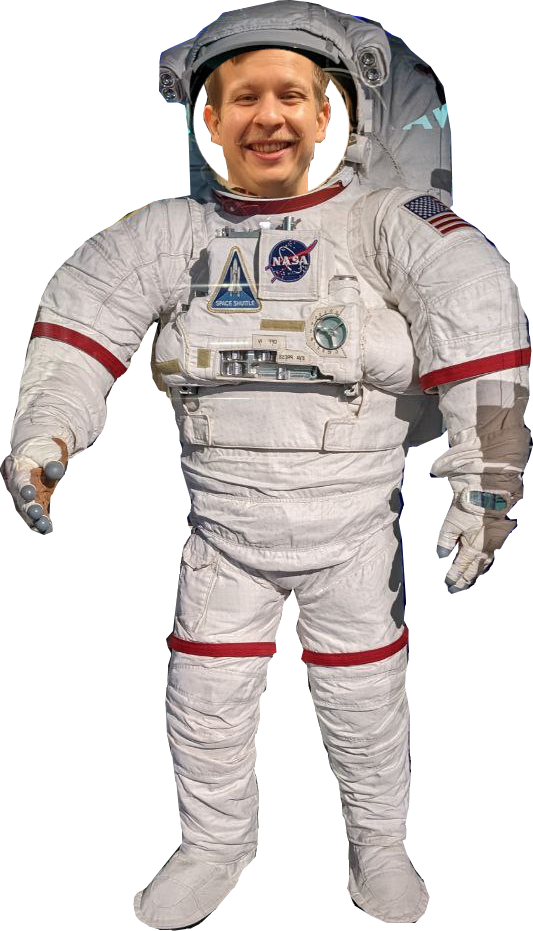
\includegraphics[height=18cm]{figures/simon4.png}
\end{center}
\section{Tomatensuppe}
\label{sec:org59a398d}
\cb{I}{ch} bin endlich wieder zurück aus dem Weltall und in meiner
Wohnung. Vor mir steht eine frische Tasse Kaffee, die Tastatur ist
bereit, der Computer wartet gerade zu meine Weihnachtsgeschichte
aufzuzeichnen. Doch dann klingelt es schon
wieder. \newline

Genervt stapfe ich los. Am Hoftor hat sich eine Menge von komisch
aussehenden Gestallten gebildet. Sie tragen Deppenmützen, die Hemden
sind voller Farbflecken und der eine oder andere hat eine Bob ross
tolle. Es sind wohl \emph{Künstler}, denke ich mir. Der Anführer dieser
elustren Gestallten schiebt sich die Nickelbrille näher an die Augen
und macht eine alberne Verbeugung zur Begrüßung. Ich habe allerdings
keine Bock mehr auf diese ständigen Störungen.

\begin{center}
"Was?!", will ich gereizt wissen.
\end{center}

\begin{center}
\grqq Es ist schräääääääcklich", beginnt der Künstler. "Sooooo
schräääääcklich!", fügt er theatralisch hinzu.
\end{center}

\begin{center}
"Junge, komm auf den Punkt!", knurre ich ihn an.
\end{center}

\begin{center}
"Wohl an. Wir sind das Künstlerkollegtiv, blauer Apfel. Und wir
haben vermommen, das ein Anschlag auf die Monalisa geplant ist",
erklärt er.
\end{center}

\begin{center}
"Lass mich raten, ich soll jetzt für euch Clowns nach Paris fahren,
und in einem Oceans 11 mässigen Heist, die Mona Lisa stehlen um sie
in Sicherheit zu bringen, und als Alibi das ganze als Städtetrip mit
meinem Kumpel Sebi ausgeben?", fasse ich zusammen.
\end{center}

\begin{center}
"Ja also, wenn das geht halt \dots{}", nickt Meister Patzig.
\end{center}

\textbf{Paris} \newline 

Ich rase mit 300Sachen im TGV Richtung Paris Gare de
l'est. Angekommen in Paris will ich direkt erstmal eine Kaffee
trinken und tappe direkt in das erste Fettnäpfchen. Das Cafe in das
ich stolpere, und ganz allgemein Cafes in Paris sind im Prinzip alle
Restaurants. Was ich gebraucht hätte wäre ein Salon de The - ein
Teehaus gewesen. 1stunde und 25Euro später verlasse ich das Cafe in
Richtung Hotel. Das Metro System in Paris ist klasse, man kauft sich
kleine Papiertickets, mit denen man dann wie ein Vollidiot vor den
Schranken zum Fahrbereich steht. Neben mir kommt ein junger Franzose
an, den könnte ich doch fragen wo das Ticket hin muss \dots{} und er
ist einfach über die Schranke gehüpft. Gott sei dank kommt eine
Französin afrikanischer Abstammung mit ihren multiplen Kindern an,
und ihr Mutterinstinkt löst dann mein Problem, da wo ich das ticket
rein stecken wollte kommt es raus, man muss die dinger unten rein
stecken. Auf der anderen Seite ballert Mama mich noch voll mit 10000
Worten auf Französch, ich glaub die peilt nicht, das ich so gut wie
nix verstehe. Aber die Quintessenz, das ich mein ticket nicht
wegwerfen soll hab ich gerafft - und das ist gut, weil am Ziel ist
wieder eine schranke, und durch die komm ich nur durch mit dem
Ticket. \newline

Das Hotel, das wir Helden uns vor allem wegen der Nähe zum Luft und
Raumfahrt Museum ausgesucht haben ist in einer eher herunter
gekommenene Ecke der Stadt. Natürlich enttäusche ich auch hier
wieder mit meiner Geniallität, denn zum einchecken braucht man eine
Kreditkarte, und für eine Kreditkarte braucht man einen Pin und wer
hat seinen Pin vergessen, genau der Simon. Als ich den Pin dann
glücklicherweise per Kreditkarten app ändern und einchecken kann,
geht es direkt zurück in die Stadt - der schweine teure Museums pass
muss sich ja lohnen. \newline 

Als Sebi dann per Bus angekommen ist, kucken wir uns direkt den
Eifelturm bei Nacht an - so romantisch. Für teuer Geld holen wir und
in einem Kiosk in der nähe ein winziges Bier und genießen dann die
Lightshow. Im Anschluss geht das nächste Abenteuer los - Sebi ist
Veganer, und in Paris, spontan um 22uhr was veganes zum Essen zu
finden stellt sich als verhältnismäsig tricky heraus. Unsere
Feldstudie ergibt zu dem, das MC Donalds in Frankreich abgesehen von
Pommes und Bier keine Veganen Burger oder ähnliches im Sortiment
führt. Schließlich steht noch die Heimreise zum Hotel an. Wie
richtige Einheimsiche der niedrigen Einkommensschichten stehen wir
in einem übervollen Bus, der uns in unsere Ghetto
bringt. \newline

Der nächste Tag ist auch wieder voll mit Abenteuer und
Excitement. Nach einem Frühstück aus der Patesserie - Baguette und
Cafe geht es los richtung Flughafen. Das Luft und Raumfahrtmuseum
liefert was es verspricht. Einzig wenn man auch in die Cockpits
gehen könnte wäre es noch besser. Freitag abend ist der Tag an dem
der Louvre länger offen hat, was wir natürlich nicht bewusst geplant
hatten, aber bei unserer Verplantheit verhindert, das wir nicht nur
1std sondern 4std im riesigen Museum verbringen können. Dieses mal
hab ich vorher geplant und wir sind erst in einem veganen Burger
restaurant und dann in einer fancy Weinschenke - Gottes
Trauben. \newline

Ganz ohne Kopfschmerzen am nächsten Tag checken wir aus dem Hotel
aus, bzw glauben wir das. Sebi wird am Abend noch einen liebevollen
Anruf der Hotel lobby bekommen - die ja eigentlich alle unsere infos
und daten haben, aber trotzdem dachten wir wollten die Zeche prellen.
Ich bin dann noch bis zum Abend in Paris, erst im Armee museum, dann
zu einem späten Frühstück und schließlich in Versailles. Selbst
verständlich schaffe ich es auch in den letzten Stunden noch einige
Male mich doof anzustellen. So komme ich in Versailles an, aber
nicht durch die Schranken im Bahnhof durch - ich bin unwissentlich
schwarz gefahren. Wenn man in Paris ein ticket kauft kommt man durch
die Schranken in den Gleisbereich, aber im Selbigen, kann man den
falschen Zug nehmen, und dann steckt man fest. Um so lustiger ist es
wenn man Simon, heißt, weil dann schafft man dass nicht nur nach
sondern auch mit dem Zug von Versailles. Zurück in Paris, stehe ich
wie ein absoluter Vollidiot an den verschlossenen Schranken. Eine
junge Frau, steht heulend auch vor den Schranken - auf Nachfrage ja
auch sie kommt nicht raus. Irgendwann finde ich dann eine Schranke
die kaputt ist und through I go. \newline 

Zum Abschluss will ich mir am Bahnhof noch ein Bier kaufen - die
Zugfahrt die mir bevor steht dauert regulär 6std, wegen Ausfällen
voraussichtlich 8std. Meine Bestellung von 3große Bier, und
1Sandwich wird zu 3Bier, 3Sandwiches im Kopf vom Bistro dude -
scheinbar ist die Vorstellung das 1Mensch 3Bier kauft zu
abwegig. Der TGV verlässt schließlich Paris. In Stuttgart ist dann
erstmal Ende. Ein französisches Pärchen, die ihren Umzug nach
München per Zug durchführen, sind dankbar um meine tragenden
Hände. Schließlich und endlich komme ich in München an. Wir tragen
das Gepäck von den beiden noch durch den ganzen Münchner
Hauptbahnhof. Im Rewe um 1uhr morgen kaufe ich noch Mehl und Bier
aber zuhause sehe ich hätte sogar noch was
gehabt. \newline

Ich rolle die Mona Lisa aus und klebe sie mit Panzertape an meine
Wand. Umwelt schutz in allen Ehren, aber in wie fern reduziert suppe
auf gemälde werfen denn Treiphausgase?

\begin{center}
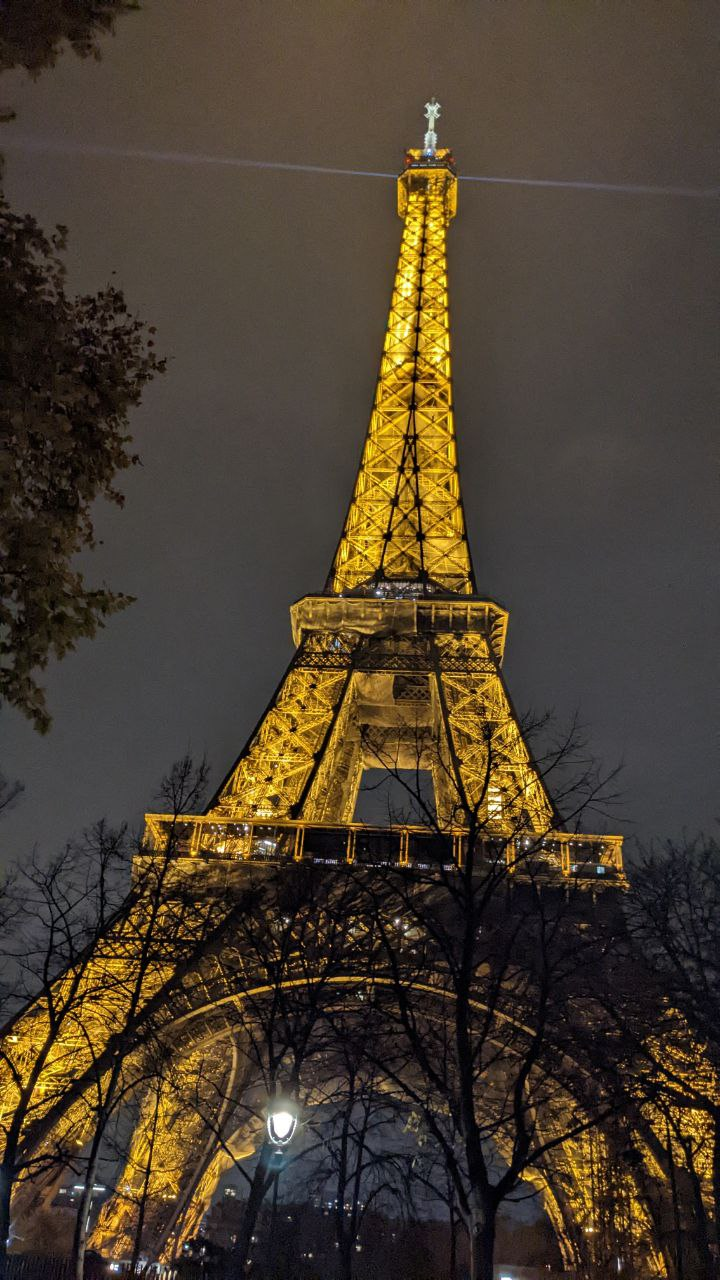
\includegraphics[height=18cm]{figures/eifel.png}
\end{center}
\section{In den Bergen}
\label{sec:org4ee2764}
\cb{N}{ach} dem aufregenden Trip in der Stadt der Liebe kann ich nun
ja endlich meine Weihnachtsgeschichte schreiben. Ich sitze, ich habe
Kaffee, ich hab Computer. Und mein Handy leutet. Mein gute Freundin
Yumi ruft an. Die hat Geburtstag und daher müssen wir alle über das
Wochenende leider nach Italien fahren, was für ein
Jammer. \newline

Natürlich fahren wir früh am Freitag los, damit wir gut bei
Tageslicht in Italien ankommen, und auf der Fahrt geht nix
schief. Als wir um 16uhr in Landshut aufbrechen ist es immerhin noch
nicht dunkel. Außerdem regnet es nicht, noch nicht. Vor Österreich
machen wir halt an einer Raststätte um die Vignette zu kaufen - aber
das geht nicht. Weil dafür verlangen die lieben Leute in der
Raststätte den Fahrzeugschein. Und weil mein Auto nur ganzjahres
Reifen hat, war mein Vater so lieb mir sein Auto zu leihen, aber wo
der Fahrzeugschein sich befindet finde ich erst 2Tage später
heraus. Es muss also die Online Vignette sein, die ist ja auch nur
doppelt so teuer wie die aus der Raststätte. Und natürlich hat das
Computersystem bei genau uns einen Fehler. Per E-Mail hält man uns
auf dem laufend, das die Bezahlung zwar schon eingegangen, die
Vignette allerdings noch nicht gültig sei - während die Grenze immer
näher kommt. Kurz davor löst sich dieser Krimi zum Glück in
Wohlgefallen auf. \newline 

Nach einem Stop für eine lecker Pizza, der ersten von vielen, kommen
wir in der Nacht im Bergdorf Pejo an. Wir fahren langsam die
kurvigen Straßen lang während die Italiener und netterweise von
hinten Lichthupe geben, damit wir besser die Straße sehen. Hirsche,
Rehe und vereinzelte Vespas kreuzen unseren Weg. In der Unterkunft
angekommen heißt es dann endlich schlafen. Am nächsten Morgen
genieße ich die warme Morgensonne auf dem Hotel balkon, der teuere
Kaffee schmeckt ausgezeichnet, die ciabatta sind frisch. Mittags
brechen wir dann auf - eine Winter und Nachtwanderung steht uns
bevor. Weil ich so unfassbar stark bin reiße ich beim Verlassen die
Türklinge vom Appartment ab. \newline

Nach der obligatorischen Pizza und Pasta Speißung gönnen wir uns
noch die eine oder andere Flasche Wein im Quartier am Abend. Am
nächsten Morgen verlassen wir dann gut gelaunt Pejo richtung
Dolomiten, aber nicht ohne zuvor einen kurzen Abstecher zu einem
Bergsee zu machen. Über schnee bedeckte Serpentinen kämpfen wir uns
langsam nach oben. Natürlich haben wir auch diese mal wieder keine
Wanderstöcke mit genommen, weil wir ja so krass sind. Schließlich
erreichen wir den Gipfel, und durch ein finsteres Loch im Berg
stehen wir vor dem Wasser. Mir ist scheiß kalt, aber ich will Yumi
ja nicht die Freude am Bergsee verderben. Ihr ist auch scheiß kalt,
aber sie denkt ich will umbedingt am See stehen bleiben. Weil wir
dumm sind, frieren wir also noch 10minuten bis es wirklich nicht
mehr geht und gehen zurück zum Auto - ein hoch auf die Sitzheizung.

\begin{center}
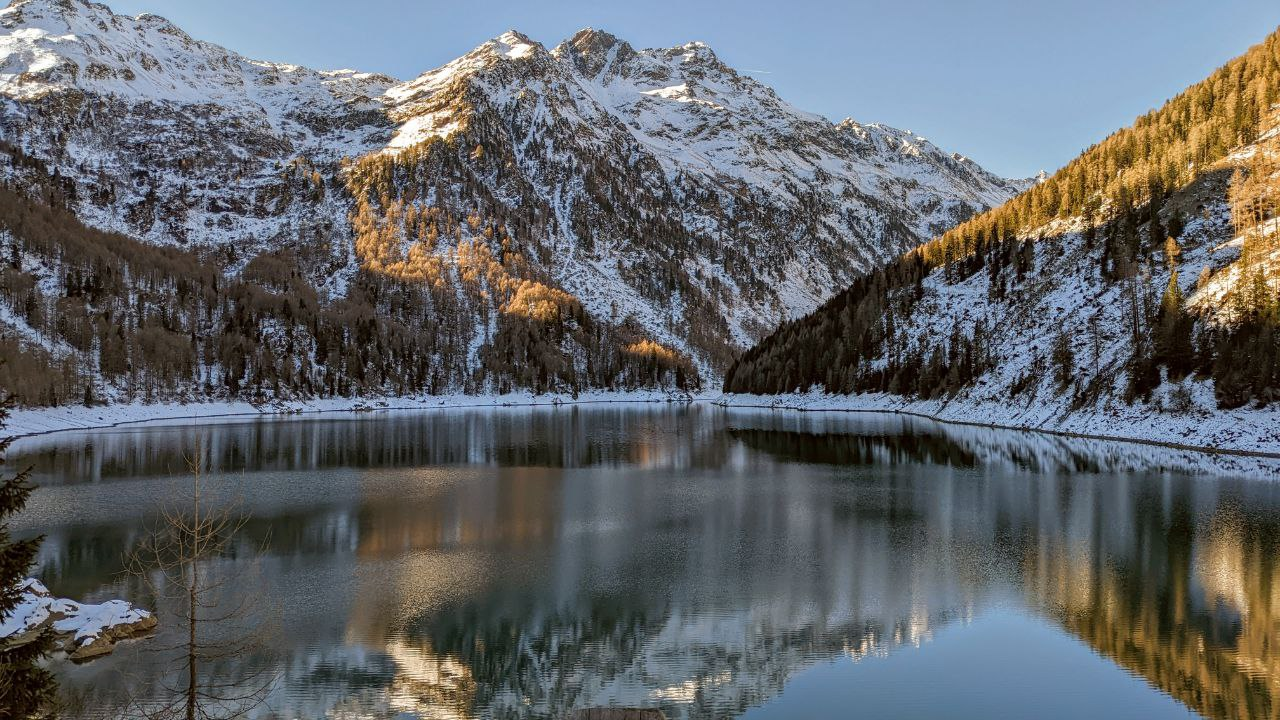
\includegraphics[width=15cm]{figures/see.png}
\end{center}

In der nähe der Dolomiten gibt es dann die finale Pizza. Über das
schöne Landshut geht es dann schließlich und endlich wieder nach
Hause.
\section{Christkind}
\label{sec:org87e7824}
\cb{E}{ndlich} sitze ich wieder zu Hause. Endlich kann und werde ich
meine Weihnachtsgeschichte schreiben. Nix und niemand kann mich
jetzt noch stoppen \dots{} ein schrilles Leuten zerreist die
Stille. Wut entbrannt reiße ich die Tür auf, nur um davor unzählige
Gestallten zu erblicken. Ein dicker Mann mit roten Mantel tritt
durch meine Tür, eine Hexe mit rollenden Augen kommt herein. Drei
heilige Könige watscheln rein, Papa Noel tritt ein. Es dauert eine
ganze Weile und meine winzige Wohnung füllt sich mehr und mehr mit
allen möglichen alten weißen Cis man personifikationen von
Weihnachten. Da ist Krampus, da drüben Nikolaus von Myra und da der
CocaCola Weihnachtsmann. Sogar Dun Che Lao Ren aus China ist
da. Einer der vielen Nikoläuse erkärt mir schließlich:

\begin{center}
"Wir wissen, das du sehr beschäftigt bist Simon. Wir sind alle
Weihnachtsmänner", die Hexe ruft dazwischen "\text{U}nd Frauen",
"\text{U}nd Frauen", ergänzt der Redner, "Der Welt."
\end{center}

Ich sehe mich im engen Raum ungläubig um.

\begin{center}
"\text{A}lle Weihnachtsmänner?", frage ich.
\end{center}

\begin{center}
"Naja, okay ein paar haben wir am Nordpol gelassen, die basteln
Geschenke", rudert der Redner zurück. 
\end{center}

\begin{center}
"\text{U}nd was wollt ihr von mir?", will ich wissen. 
\end{center}

\begin{center}
"Das nürnberger Christkind hat einen Schnupfen und die Grippe weil
du Hyperspreader wieder zu Sebastian fahren musstest!", schimpft
mich die italienische Weihnachtshexe zusammen.
\end{center}

\begin{center}
"\text{U}nd deswegen musst du jetzt für sie einspringen und in
Bayern die Weihnachtsgeschenke verteilen", erklärt Casper, der
heilige König.
\end{center}

\begin{center}
"Hier ist das Kostüm, mit den Zeitreiseraketenrucksack, deine
Schicht fängt in 20minuten an", fügt Melchior hinzu, während
Baltasar in meinem Badezimmer verschwindet.
\end{center}

\begin{center}
"\text{A}ber das nürnberger Christkind ist doch ein Mädchen", wende
ich ein.
\end{center}

\begin{center}
"\text{U}nd Jesus war ein Junge \dots{} jetzt stell dich nicht so an!"
\end{center}

Wenn ihr also gerade bei der Beschehrung sitzt dann wisst ihr jetzt
wer euch die Geschenke gebracht hat, ich. Vorausgesetzt ihr wohnt in
Bayern, sonst kommt die Hexe!

\newpage

\begin{center}
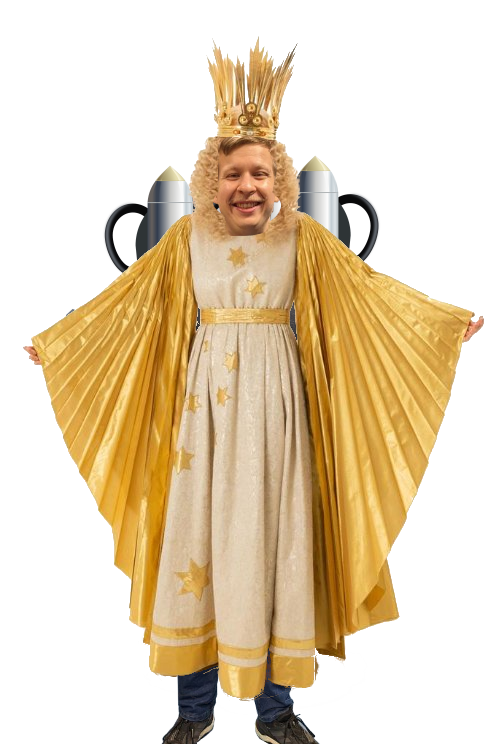
\includegraphics[height=14cm]{figures/simon5.png}
\end{center}

\begin{center}
Ich wünsche dir und euch \\
eine besinnliche Weihnachtszeit mit mega vielen Geschenken \\
und leckerem Essen und viel Freude.

Fröhliche Weihnachten, dein Simon.
\end{center}
\section{Schlusswort}
\label{sec:org51c64d3}
So liebe Leute, das war es schon wieder mit meiner
Weihnachtsgeschichte für dieses Jahr. Den Umständen geschuldet war
es dieses Jahr etwas stressiger und die Welt konnte ich auch nur 1-2
mal retten. Deutlich seltener als üblich. Aber ihr wisst ja wie es
ist - es gibt immer ein neues Jahr, eine neue Weihnachtsgeschichte,
ein neues Abenteuer. In diesem Sinne:

\begin{center}
Fröhliche Weihnachten und ein guter Rutsch in das neue Jahr.\\
Und wer an Silvester noch nichts vor hat, Party in Sebastians haus,
ich hab die Bude, weil ich auf den Hund aufpasse \dots{}
\end{center}
\end{document}